
% %%%%%%%%%%%%%%%%%%%%%%%%%%%%%%%%%%%%%%%%%%%%%%%%%%%%%%%%%%%%%%%%%%%%%%%%%%%%%
% 在这里填入题目
% %%%%%%%%%%%%%%%%%%%%%%%%%%%%%%%%%%%%%%%%%%%%%%%%%%%%%%%%%%%%%%%%%%%%%%%%%%%%%
\def\sectionName{字符串 - 字典树}



% 如果它是 beamer
\if 1\isBeamerMode\relax
    \section[\TOCName]{\sectionName}
\fi
% 如果它是 paper
\if 0\isBeamerMode\relax
    \section[\TOCName\ -\ \sectionName]{\sectionName}
\fi

\begin{frame}

% 如果它是 beamer
\if 1\isBeamerMode\relax
    \noindent {\Huge \sectionName}\par
\fi

% %%%%%%%%%%%%%%%%%%%%%%%%%%%%%%%%%%%%%%%%%%%%%%%%%%%%%%%%%%%%%%%%%%%%%%%%%%%%%
% 在这里填入你的名字
% %%%%%%%%%%%%%%%%%%%%%%%%%%%%%%%%%%%%%%%%%%%%%%%%%%%%%%%%%%%%%%%%%%%%%%%%%%%%%
\sectionAuthor{Ding Yuyang}



% %%%%%%%%%%%%%%%%%%%%%%%%%%%%%%%%%%%%%%%%%%%%%%%%%%%%%%%%%%%%%%%%%%%%%%%%%%%%%
% 这里可以写感想(嘲讽,bushi),也可以不写!!!
% %%%%%%%%%%%%%%%%%%%%%%%%%%%%%%%%%%%%%%%%%%%%%%%%%%%%%%%%%%%%%%%%%%%%%%%%%%%%%
\noindent 字典树是字符串算法中比较基础的算法之一。



\end{frame}

% %%%%%%%%%%%%%%%%%%%%%%%%%%%%%%%%%%%%%%%%%%%%%%%%%%%%%%%%%%%%%%%%%%%%%%%%%%%%%
% 这里开始写简单的题目意思 ~
% %%%%%%%%%%%%%%%%%%%%%%%%%%%%%%%%%%%%%%%%%%%%%%%%%%%%%%%%%%%%%%%%%%%%%%%%%%%%%
\subsection{字典树状态}
\begin{frame}{字典树的形态举例} % 如果一个 frame 写不下的话,多开几个就好了~
比如含有 and, as, at, cn, com 的字典树:
\begin{center}
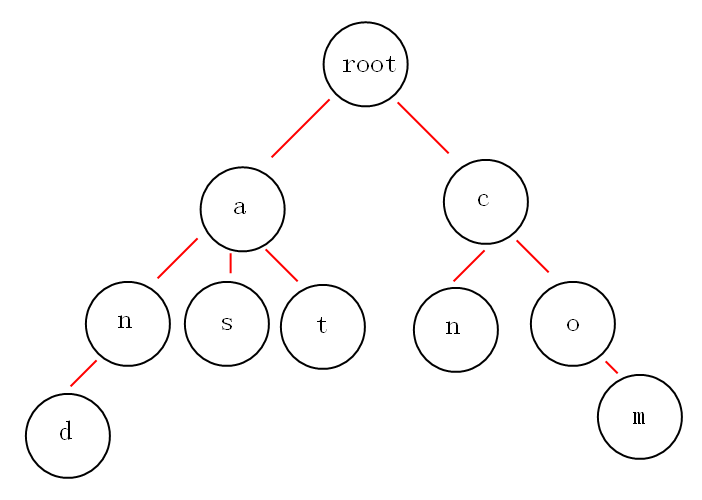
\includegraphics[width=0.7\textwidth]{./pic/trie_state.png}
\end{center}
\end{frame}

\begin{frame}
\begin{itemize}
    \item 根节点不包含字符,除根节点外的每一个子节点都包含一个字符。
    \item 从根节点到某一节点,路径上经过的字符连接起来,就是该节点对应的字符串。
    \item 每个单词的前缀作为一个字符节点保存。
\end{itemize}
\end{frame}

\begin{frame}[fragile]{新建节点}
时间复杂度: $O(|\sum|)$, 其中 $\sum$ 是字符集。

\begin{lstlisting}[language=C++]
int newnode(void) {
    ++num;
    color[num] = 0;
    cnt[num] = 0;
    memset(tree[num], 0, sizeof(tree[num]));
    return num;
}
\end{lstlisting}
\end{frame}

\begin{frame}[fragile]{字典树的插入操作}
\begin{lstlisting}[language=C++]
void insert(char s[]) {
    int n = strlen(s), p = 0;
    for (int i = 0; i < n; i++){
        int c = s[i] - 'a';
        if (tree[p][c] == 0) tree[p][c] = newnode();
        p = tree[p][c];
        cnt[p]++;
    }
    color[p]++;
}
\end{lstlisting}
\end{frame}

\begin{frame}[fragile]{字典树的查找操作}
\begin{lstlisting}[language=C++]
int find(char s[]) {
    int n = strlen(s), p = 0;
    for (int i = 0; i < n; i++){
        int c = s[i] - 'a';
        if (tree[p][c] == 0) return 0;
        p = tree[p][c];
    }
    return color[p];
}
\end{lstlisting}
\end{frame}

\subsection{做题}
\begin{frame}{做题}
TODO。
% \begin{itemize}
%     \item HDU - 1251。
% \end{itemize}
% \end{frame}
% 
% \begin{frame}
% \begin{itemize}
%     \item 给定一个 $n$ 个数的数组 $a$, 满足 $1\leq n\leq 10^5, 0\leq a_i\leq
%         10^9$。
%     \item 现在询问 $m$ 次,每次给出一个数 $x$, 数组中与 $x$ 异或值最大的数是多少。
%         $1\leq m\leq 10^5$。
% \end{itemize}
% \end{frame}
% 
% \begin{frame}
% \begin{itemize}
%     \item 暴力复杂度: $O(nm)$
%     \item 怎么用字典树?
% \end{itemize}
% \end{frame}
% 
% \begin{frame}
% \begin{center}
% 01trie + 贪心
% \end{center}
% \end{frame}
% 
% \begin{frame}
% \begin{itemize}
%     \item 提高难度
%     \item 对于 $n$ 个数的数组,球最大区间异或和
%     \item 区间 $(l, r)$ 的区间异或和为 $a[l]\oplus a[l + 1]\oplus ...\oplus a[r]$
% \end{itemize}
\end{frame}

